\documentclass[a4paper,12pt]{article}
\usepackage[utf8]{inputenc}
\usepackage{cludein}
\usepackage{xcolor}
\usepackage[toc,page]{appendix}
\usepackage{algorithm2e}
\definecolor{light-gray}{gray}{0.5}
% Definindo novas cores
\definecolor{verde}{rgb}{0.25,0.5,0.35}
\definecolor{jpurple}{rgb}{0.5,0,0.35}
% Configurando layout para mostrar codigos Java
\usepackage{listings}
\DeclareGraphicsExtensions{.pdf,.png,.jpg}
\lstset{
  language=Java,
  basicstyle=\ttfamily\small, 
  keywordstyle=\color{jpurple}\bfseries,
  stringstyle=\color{red},
  commentstyle=\color{verde},
  morecomment=[s][\color{blue}]{/**}{*/},
  extendedchars=true, 
  showspaces=false, 
  showstringspaces=false, 
  numbers=left,
  numberstyle=\tiny,
  breaklines=true, 
  backgroundcolor=\color{cyan!10}, 
  breakautoindent=true, 
  captionpos=b,
  xleftmargin=0pt,
  tabsize=4
}
\pagestyle{plain}
\pagenumbering{arabic}
\usepackage[portuguese]{babel}
\addto\captionsportuguese{
\renewcommand{\figurename}{Fig.}
\renewcommand{\tablename}{Tab.}}
\begin{document}
\title{Relatório de Implementação dos Algoritmos Referente ao Problema da Árvore Geradora Mínima}
\author{Bruno Ramos \and Madson Araújo \and Nemuel Leal \and Nilton Vasques}
\date{\today}
\maketitle

\section{Definição}
Seja G=(V,E) um grafo não direcionado e conexo, G'=(V,E') é chamado de subgrafo gerador se possuí os mesmos vértices de G. Portanto se tivermos em G' uma árvore, então o subgrafo é uma árvore geradora. 
Quando G é um grafo conexo, em que cada aresta possui um valor ou peso p(e), o peso total da árvore geradora é \[\sum_{e \in E'}p(e)\] onde p(e) é uma função que retorna o peso da aresta \emph{e}. Á árvore geradora mínima é a árvore G' que possui o menor peso total dentre todas as árvores possíveis do grafo G\cite{nogueira}. Podemos enunciar a função para encontrar a árvore geradora mínima como \[\emph{min}\sum_{e\in E'}p(e)\].
A partir dessa noção podemos visualizar que encontrar a árvore geradora mínima não é tão trivial assim. Se propormos uma solução pela força bruta, ou seja, encontrar todas as árvores geradoras e assim então verificar qual a que possui o menor peso total. No pior caso quando temos um grafo completo(em que todos os vértices se ligam uns aos outros) teríamos $n^{n-2}$ árvores geradoras onde n é o número de nós, sendo assim teríamos uma solução em tempo exponencial $O(n^n)$ e inviável \nocite{*}.
Diante deste cenário alguns matemáticos elaboram soluções para o problema das Árvores Geradoras Mínimas, se utilizando de heurísticas gulosas para encontrar a solução ótima. No presente artigo abordaremos o Algoritmo de Kruskal e o de Prim, como estudo de caso.

\subsection{Algoritmo de Kruskal}
O algoritmo de Kruskal é um algoritmo guloso, que tem por objetivo encontrar uma árvore geradora mínima para um grafo conexo e valorado ( com pesos nas arestas ). Vale ressaltar que para árvores não conexas, o algoritmo encontra floresta geradora mínima, ou seja uma árvore geradora mínima para cada componente conexo do grafo. O algoritmo pode ser enunciado nos seguintes passos:

\begin{algorithm}[H]
\SetAlgoLined
\KwData{ Um grafo Conexo }
\KwResult{ Uma árvore geradora mínima a partir de um grafo conexo }
Criar uma floresta \emph{F}, onde cada vértice do grafo é uma árvore separada\;
Criar um conjunto \emph{S} contendo todos as arestas do grafo\;
\While { \emph{S} é não vazio}{
	Remova um aresta \emph{e} com peso mínimo de S\;
	Se \emph{e} conecta duas diferentes árvores, então adicione \emph{e} para floresta \emph{F}\;
	Caso contrário, discarte \emph{e}, ou seja se a escolha de \emph{e} gera um circuito em \emph{F}, discarte-a\;
}
\caption{Pseudo Código do algoritmo de Kruskal}
\end{algorithm}

\subsubsection{Implementação}
A implementação foi realizada em Java com uso da estrutura de dados de listas encadeadas para manipular os conjuntos disjuntos. O código fonte está disponível no Apêndice A. A seguir o pseudo código da implementação com as manipulações representadas pelas operações Union-Find :\\
\begin{algorithm}[H]
\LinesNumbered
\SetAlgoLined
\KwData{ V, E}
\KwResult{ A, W}
W $\gets$ 0; A $\gets$ vazio\;
\For{ $v \in V $ }{
	$ a[v] \gets\textbf{{\color{blue}make-set}(v)}$\;
}
$L \gets \textbf{ordene}(E ,w )$\;
$k \gets 0$\;
	\While{ $k \neq \mid V\mid-1$ }{
	\textbf{remove}(L, (u, v ))\;
	a[u] $\gets$ \textbf{{\color{blue}find-set}(u)}\; 
	a[v] $\gets$ \textbf{{\color{blue}find-set}(v)}\;
	\If{ $a[u] \neq a[v]$ }{
		$aceita (u,v)$\;
		$A \gets A \cup \{(u, v )\}$\;
		$W \gets W + w (u, v )$\;
		$k \gets k + 1$\;
	}
	$\textbf{{\color{blue}union}}(a[u], a[v])$\;
}
$\textbf{retorne} (A, W)$\;
\caption{Pseudo Código do algoritmo de Kruskal com UnionFind}
\end{algorithm}

\subsubsection{Análise de Complexidade}
A estrutura de dados UnionFind mantém um conjunto de elementos particionados em vários subconjuntos não sobrepostos. O algoritmo que controla essa estrutura possui duas operações principais:
\begin{itemize}
\item Find: Determina de qual subconjunto um elemento pertence.
\item Union: Faz a união de dois subconjuntos em um só subconjunto.
\end{itemize}

A ordenação na linha 5 tem complexidade \emph{ $\Theta( \mid E\mid log \mid E\mid )$ } e domina a complexidade das demais operações.
A repetição das linhas 7-17 será executado \emph{$\Theta(\mid E\mid)$} no pior caso.
Logo, a complexidade total das linhas 9-10 será \emph{$\Theta(\mid E\mid f(\mid V\mid))$}, onde $f(\mid V\mid))$ é complexidade da função \textbf{{\color{blue}find-set}}.
As linhas de 12 a 15 serão executados $\mid V\mid -1$ vezes no total, pois para um grafo contendo N vértices, precisamos de apenas N-1 arestas para interligar todos os nós e gerar uma árvore geradora mínima. 
Assim, a complexidade total de execução destas linhas será \emph{ $\Theta(\mid V\mid . g(\mid V\mid)$} onde $g(\mid V\mid)$ é a complexidade de realizar \textbf{{\color{blue}union}}.
A complexidade do algoritmo de Kruskal será então: \[ \emph{ $\Theta(\mid E\mid log \mid E\mid + \mid E\mid .f(\mid V\mid) + \mid V\mid . g(\mid V\mid)) $}\]
A estrutura de dados UnionFind foi implementada na sua forma simples, com o uso de uma lista encadeada. Sendo assim a complexidade da função find é \emph{$\omega(n)$}, e union tem complexidade \emph{$\Theta(n)$} \cite{Cormem}. A complexidade final da implementação foi:
\[ \emph{ $\Theta(\mid E\mid log \mid E\mid + \mid E\mid .\Omega(\mid V\mid) + \mid V\mid . \Theta(\mid V\mid)) $}\]

A complexidade pode ser reduzida utilizando de uma estrutura de dados mais refinada para implementar a manipulação dos conjuntos disjuntos, como por exemplo usar uma lista encadeada e \emph{weighted-union heuristic}\cite{Cormem}, consegue-se uma complexidade de \emph{$\Theta(m+nlogn) $} para realizar as \emph{m} operações de \textbf{{\color{blue}make-set}}, \textbf{{\color{blue}find-set}} e \textbf{{\color{blue}union}} \cite{Cormem}.
\newpage
\subsection{Algoritmo de Prim}
Assim como o algoritmo de Kruskal's o algoritmo de Prim utilizada também uma heurística gulosa para solucinar o problema da Àrvore Geradora Mínima. A heurística utilizada é procurar o caminho mais curto, dentre todos os possíveis, de maneira similar ao algoritmo de Djikstra. O algoritmo de Prim's tem uma propriedade de que as arestas em \emph{A} sempre forma uma árvore simples \emph{Fig.1}.

\begin{figure}[h!]
	\caption{Ilustração do Algoritmo de Prim}
	\centering
	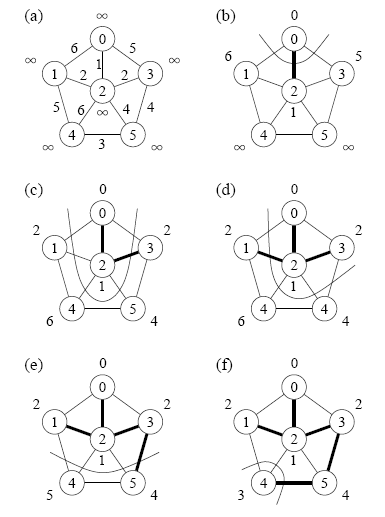
\includegraphics[width=0.5\textwidth]{prim}
	\label{fig:prim_fig}
\end{figure}

O algoritmo genérico de Prim procura encontrar o caminho mais curto de um vértice para os vértices vizinhos, até que todos os vértices estejão ligados uns aos outros. O pseudo-código pode ser visualizado logo abaixo:

\begin{algorithm}[H]
\SetAlgoLined
\KwData{ Um grafo Conexo }
\KwResult{ Uma árvore geradora mínima a partir de um grafo conexo }
Escolha um vértice S para iniciar o subgrafo\;
\While { há vértices que não estão no subgrafo }{
	selecione uma aresta segura\;
	insira a aresta segura e seu vértice no subgrafo\;
}
\caption{Pseudo Código do algoritmo de Prim}
\end{algorithm}

\subsubsection{Implementação}
Assim como a implementação anterior o algoritmo de Prim's foi implementado em Java e fez uso da Matriz de Adjacências Binária como estrutura de dados para armazenar os vértices adjacentes de um dado vértice u.  O código fonte está disponível no Apêndice A. O pseudo código que foi utilizado para a implementação pode ser visualizado em \emph{Algorithm 4}.

\begin{algorithm}[H]
\LinesNumbered
\SetAlgoLined
\KwData{ V, E}
\KwResult{ A, W}
dist[r] $\gets$ 0;
Q $\gets$ V\;
\For{ $v \in V-\{r\} $ }{
	$ dist[r] \gets \infty $\;
}
$ pred[r] \gets NULL$\;
$ A \gets \emptyset$\;
$ W \gets 0$\;
\While{  Q não for vazio  }{
	remover de Q o vértice u com menor valor em dist\;
	$ W \gets W + dist[u] $\;
	\If{ $ pred[u] \neq null $ } {
		$ A \gets A \cup \{(pred[u],u\}$\;
	}
	\For{ $ v \in Adj[u] $ }{
		\If{$v \in Q$ and $dist[v] > w[u,v] $} {
			$ dist[v] \gets w[u,v] $\;
			$ pred[v] \gets u $\;
		}
	}
}
$\textbf{retorne} (A, W)$\;
\caption{Pseudo Código do algoritmo de Prim}
\end{algorithm}

\subsubsection{Ánalise de Complexidade}

A complexidade do algoritmo de Prim está diretamente ligada a maneira de como é implementada a estrutura de dados em Q. Uma simples implementação utilizando matrizes de adjacência vai requerer complexidade \emph{$\Theta(\mid V\mid^2)$} e foi a estrutura de dados utilizada neste trabalho. Utilizando de uma heap binária a complexidade cai para \emph{$\Theta(\mid E\mid log\mid V\mid)$}, ainda assim é possível decrescer ainda mais a complexidade utilizando como estrutura de dados uma Fibonacci Heap com complexidade \emph{$\Theta(\mid E\mid+\mid V\mid log\mid V\mid)$} \cite{Cormem}.


\appendix
\begin{appendices}
\section{\\Algoritmos Implementados no Projeto} \label{App:AppendixA}

\begin{lstlisting}[label=figura,title=Implementação do Algoritmo de Kruskal em Java]
public class Kruskal implements GraphAlgorithm{
	private Graph mGraph;
	private int edges[];
	private int edgeIndex = 0;
	
	public Kruskal(Graph grafo) {
		mGraph = grafo;
	}	

	@Override
	public void init(){
		edgeIndex = 0;
		for (int i = 0; i < mGraph.getVerticesCount() ; i++) {
			Vertice vertice = mGraph.getVertices()[i];
			UnionFind.makeSet(vertice);
		}
		edges = new int[mGraph.getArestasCount()];
		for( int i = 0; i < edges.length; edges[i] = i++);
		qsort(0, edges.length -1);
	}
	@Override
	public boolean performStep() {
		if( edgeIndex >= edges.length )
			return true;
		Aresta aresta 	= mGraph.getArestas()[ edges[edgeIndex]];
		if( aresta.status == Status.WAITING ){
			aresta.status = Status.PROCESSING;
			return false;
		}
		edgeIndex++;
		UnionElement u 	= aresta.u;
		UnionElement v 	= aresta.v;
		if( !UnionFind.find(u).equals(UnionFind.find(v))){
			aresta.status = Status.TAKED;
			UnionFind.union(u, v);
		}else{
			aresta.status = Status.DISCARDED;
		}
		return false;
	}
}
\end{lstlisting}

\begin{lstlisting}[title=Implementação do Algoritmo de Prims em Java]
public class Prim implements GraphAlgorithm{
	private Graph mGraph;
	private AdjacencyMatrix verticesMatrix;
	private AdjacencyMatrix matrix;
	private boolean processing = false;

	public Prim( Graph graph) {
		mGraph = graph;
	}
	@Override
	public void init() {
		processing = false;
		verticesMatrix = new AdjacencyMatrix(mGraph.getVerticesCount());
		verticesMatrix.makeAdjacency(0, 0);
		matrix = mGraph.createAdjacencyMatrix();
	}

	@Override
	public boolean performStep() {
		Aresta bestChoice 	= null;
		int bestVertice 	= -1;
		int vertices[] = verticesMatrix.getAdjacencys(0);
		for( int v = 0; v < vertices.length; v++){
			if( vertices[v] == 1){
				int adjacencys[] = matrix.getAdjacencys(v);
				for( int i = 0; i < adjacencys.length; i++){
					if(adjacencys[i] == 1){
						Aresta aresta = mGraph.getAresta(i, v);
						if( aresta != null){
							if( !processing ){
								aresta.status = Status.PROCESSING;
							}else if ( bestChoice != null ){
								if( bestChoice.weight > aresta.weight ){
									bestChoice  = aresta;
									bestVertice = i;
								}
							}else{
								bestChoice = aresta;
								bestVertice = i;
							}
						}
					}
				}
			}
		}
		if(!processing){
			processing = true;
			return false;
		}
		boolean finish = true;
		if( bestVertice != -1 ){
			bestChoice.status = Status.TAKED;			
			for(int i = 0; i < vertices.length; i++){
				if( vertices[i] == 1){
					matrix.removeAdjacency(i, bestVertice);
				}else{
					finish = false;
				}
			}			
			processing = false;
			verticesMatrix.makeAdjacency(0, bestVertice);
		}
		return finish;
	}


}
\end{lstlisting}

\section{\\Código Fonte das Estrutura de Dados Implementadas no Projeto} \label{App:AppendixE}
\begin{lstlisting}[title=Interface Para Operações Union-Find com Lista Encadeada]
package br.ufba.datastructures;
/**
 * @author niltonvasques
 * UnionFind data structure
 * http://en.wikipedia.org/wiki/Disjoint-set_data_structure
 */
public class UnionFind {

	public interface UnionElement{

		public UnionElement getRoot();
		public UnionElement getParent();
		public void setRoot(UnionElement x);
		public void setParent(UnionElement x);

	}

	public static void makeSet( UnionElement x ){
		x.setParent(x);		
	}

	public static UnionElement find( UnionElement x){
		if ( x.getParent() == x )
			return x;
		else
			return find(x.getParent());
	}

	public static void union( UnionElement x, UnionElement y){
		x.setRoot( find(x) );
		y.setRoot( find(y) );		
		x.getRoot().setParent( y.getRoot() );
	}

}
\end{lstlisting}

\begin{lstlisting}[title=Implementação da Matriz de Adjacências Binária]
package br.ufba.datastructures;

/**
 * @author niltonvasques
 * http://pt.wikipedia.org/wiki/Matriz_de_adjac%C3%AAncia
 */
public class AdjacencyMatrix {

	private static final int MEM_BLOCK_SIZE = 32;
	int matrix[];
	int stride;
	public AdjacencyMatrix(int n) {
		stride = n;
		int size = (int)(stride * stride);
		int lenght = 1 + (size/32);
		matrix = new int[ lenght ];	
	}

	public void makeAdjacency(int element, int adjacency ){
		makeAdjacencyInternal(element, adjacency);
		makeAdjacencyInternal(adjacency, element);  
	}

	public void removeAdjacency(int element, int adjacency ){
		removeAdjacencyInternal(element, adjacency);
		removeAdjacencyInternal(adjacency, element);  
	}

	private void makeAdjacencyInternal(int element, int adjacency) {
		int bitIndex			= (element*stride+adjacency);
		int index 		= (int) (bitIndex/MEM_BLOCK_SIZE);
		int shift 		= bitIndex % MEM_BLOCK_SIZE;
		matrix[index] 	|= (0x01 << shift);
	}

	private void removeAdjacencyInternal(int element, int adjacency) {
		int bitIndex			= (element*stride+adjacency);
		int index 		= (int) (bitIndex/MEM_BLOCK_SIZE);
		int shift 		= bitIndex % MEM_BLOCK_SIZE;
		matrix[index] 	&= ~(0x01 << shift);
	}

	public int[] getAdjacencys(int element){
		int adjacencys[] = new int[stride];

		int bitIndex		= (element*stride);
		int bitRemainder	= (bitIndex % MEM_BLOCK_SIZE);

		for( int i = 0; i < stride; i++){
			int x = ((bitIndex+i)/MEM_BLOCK_SIZE);
			int y =  bitRemainder + i;

			int ret = (matrix[x] >> y) & 0x01;
			adjacencys[i] = ret;		
		}		

		return adjacencys;
	}

	public boolean checkAdjacency(int u, int v){

		int bitIndex		= (u*stride);
		int index 			= (int) (bitIndex/MEM_BLOCK_SIZE);

		int x = (v/MEM_BLOCK_SIZE) + index;
		int y = (bitIndex % MEM_BLOCK_SIZE) + v;

		return ((matrix[x] >> y) & 0x01) == 0x01;
	}
}
\end{lstlisting}

\end{appendices}

\bibliographystyle{plain}
\bibliography{biblio}

\end{document}


